\documentclass[PI,KR]{HSEUniversity}
% Возможные опции: KR или VKR; PI или BI

%%% Работа с таблицами
\usepackage{array,tabularx,tabulary,booktabs} % Дополнительная работа с таблицами
\usepackage{longtable}  % Длинные таблицы
\usepackage{multirow} % Слияние строк в таблице

\title{Разработка Информационной системы для поиска исполнителей по техническому заданию прикладного проекта}
\author{Соломатин Роман Игоревич}
\supervisor{к.т.н., доцент кафедры Информационных технологий в бизнесе НИУ ВШЭ-Пермь}{А. В. Бузмаков}
\Year{2021}
\Abstract{
	Ежедневно появляется множество тендеров, в которых можно принять учатие. Но на подготовку к нему отводистся мало времени. Данная работа посвящена проблеме поиска исполнителей по текстовому описанию тендера.
	
	В первой главе находится постановка задачи, обзор существующих решений, выбор языка программирования и системы управления базами данных.
	
	Во второй главе представлено проектирование базы данных, информационной системы и сбор данных.
	
	В третьей главе содержится описание процесса разработки информационной системы.
	
	Количество страниц – 26, количество иллюстраций – 9, количество таблиц – 3.
}

% Ссылка на файл с описание библиографии
\bibliography{library.bib}

\begin{document}

\maketitle

\chapter*{Введение}
Каждый день выкладывается несколько десятков тендеров, сроки участия в которых очень сжаты, и потенциальным исполнителям надо быстро определиться смогут ли они выполнить тендер или нет. Для принятия решения надо ознакомиться с тендером, собрать команду профессионалов для участия в заявке и выполнения тендера, а также и подготовить заявку. Это все может занять много времени. Действительно, в <<Высшей школе экономики>> много людей с разными компетенциями, и надо по текстовому описанию тендера понять, кто его сможет сделать. Для этого нужно знать, в чем каждый из работников университета компетентен. Для того чтобы узнать компетенции каждого из работников, можно проанализировать тексты, в создании которых сотрудник университета принял участие.

В рамках ВШЭ сотрудники принимают участие в создании нескольких видов текстов, в том числе статьи в научные журналы и выпускные курсовые работы, которые пишут студенты под их руководством. Анализируя эти тексты можно выделить сферы интересов сотрудников. Для целей такого анализа на первом этапе были выбраны ВКР, потому что для доступа ко многим научным журналам требуется платная подписка и кроме того различные научные статьи выложены на различных сайтах, что затрудняет единообразную работу с ними. Кроме того, статьи пишутся на разных языках, что тоже затрудняет работу. А выпускные курсовые работы, напротив, находятся в свободном доступе и при этом похожи на научные статьи и содержат много текстовой информации для получения выявление компетенций сотрудников. Таким образом, можно получить сферу компетенций сотрудника, по которой в дальнейшем искать соответствие между пришедшем текстовым описанием задачи и профилем сотрудника. Получается, есть проблемы поиска исполнителей на тендер. 

Таким образом, проблемой рассматриваемой в данной работе является автоматический поиск исполнителей под тендер, заданный текстовым описанием. В рамках работы будет проверяться гипотеза, можно ли автоматически на основании анализа текстов ВКР, написанных под руководством сотрудника НИУ ВШЭ, получить сферу компетенций преподавателя,по которой в дальнейшем искать соответствие с текстовым описанием тендера.

Объект исследования - процесс поиска исполнителей по текстовому описанию тендера.

Предмет исследования - автоматизация процесса поиска исполнителей по текстовому описанию тендера.

Цель работы – создать информационную систему для поиска исполнителя по текстовому описанию тендера.

Для достижения поставленной цели нужно сделать:

В первой главе постановка задачи.

Во второй главе описание проектирования системы.

В третьей главе пример работы приложения.

Работа оформлена в соответствии с правилами написания курсовых работ \cite{HSEDocuments}.
\chapter{Анализ предметной области}
\section{Формальная постановка задачи}
На данный момент достаточно затруднительно найти программные продукты, которые могут находить исполнителей по текстовому описанию тендера. Действительно, это нетипичная ситуация, когда есть много исполнителей с разными компетенциями, которые ограничено известны лицу, составляющему команду по заявки на тендер. Также редко в каких организациях по текстам, которые пишут исполнители можно составить представлении о их компетенциях. Сейчас это проблема решается вручную.


Через ВШЭ проходит много тендеров, задаваемых техническими заданиями. Эти заявки проходят через несколько фильтров и попадают к специальному человеку, которые принимает решение, на сколько эта заявка подходит под профиль компетенций ВШЭ. Этот человек знает компетенции многих исполнителей НИУ ВШЭ и может оценить, насколько рассматриваемый тендер может быть решён силами НИУ ВШЭ. После этого, если этот человек думает, что тот или иной исполнитель обладает требуемыми компетенциями, то ему пишется письмо. Сотрудник через некоторое время отвечает готов ли он участвовать в заявке на тендер и в его исполнении. Если удалось найти команду, то за оставшееся, обычно короткое время, нужно подготовить проект заявки, задать уточняющие вопросы организатору тендера, найти недостающих исполнителей, а также выполнить много других задач. Данный процесс занимает много времени Эта система имеет недостатки:
\begin{itemize}
	\item Много тендеров теряется, так как человек не знает все компетенции всех исполнителей
	\item Сложно искать тендеры
	\item Тяжело масштабировать, потому что необходимо знать много про разных людей
	\item Тратится много времени
\end{itemize}

Иногда применятся способ массовой рассылки требующихся исполнителей для тендера. У данного подхода также есть определённые недостатки:
\begin{itemize}
	\item Массовую рассылку не все читают
	\item Не даёт полную информацию о тендере
\end{itemize}

Целевая система работе система поможет автоматизировать следующие процессы:
\begin{itemize}
	\item Определение компетенций сотрудника
	\item Поиск сотрудников для выполнения задания
\end{itemize}
Варианты использования реализуемой системы:
\begin{itemize}
	\item Просмотр активных проектов
	\item Поиск компетенций исполнителя
	\item Подбор сотрудника для проекта
	\item Редактирование информации о исполнителя
\end{itemize}

Так как в данной работе нужно проверить гипотезу, будет разрабатываться прототип программы. Диаграмма вариантов использования конечного программного продукта показана на рисунке \ref{fig:figure2}. Ниже рассмотрим подробнее каждый из приведённых прецедентов.
\begin{FIGURE}[h]{Диаграмма вариантов использования \label{fig:figure2}}
	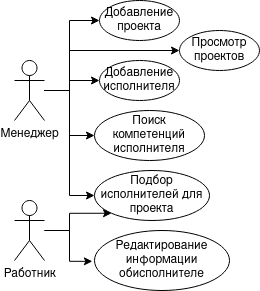
\includegraphics[width=0.6\textwidth]{img/Диаграмма вариантов использования}
\end{FIGURE}

\subsection{Прецедента <<Добавление тендера>>}
Предоставляется текстовое описание тендера и потом для него подбираются исполнители из базы данных.
\subsection{Прецедента <<Просмотр тендеров>>}
Выдаётся список тендеров, на которые были отправлены заявки об участии в тендере.
\subsection{Прецедента <<Добавление исполнителя>>}
Добавление исполнителя в базу данных, и запись данных о нем.
\subsection{Прецедента <<Поиск компетенций исполнителя>>}
Создание компетенций для заданного человека. Для этого надо обработать тексты ВКР с его профиля на сайте <<Высшей школы экономики>>, которые хранятся в формате docx, doc или pdf. \ref{fig:Find actor}
\begin{FIGURE}[h]{Поиск компетенций исполнителя \label{fig:Find actor}}
	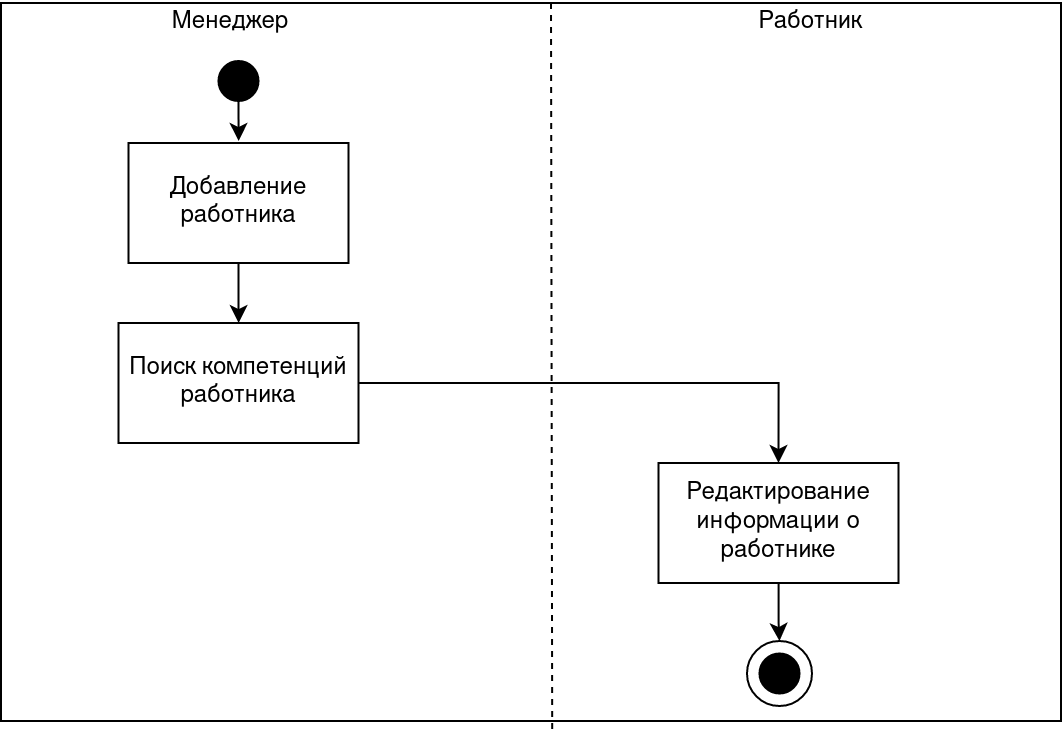
\includegraphics[width=0.6\textwidth]{img/Диаграмма Бизнес-процесса 2}
\end{FIGURE}
\subsection{Прецедента <<Подбор исполнителя для тендера>>}
Подбор исполнителя под текстовое описание тендера. \ref{fig:figure1}
\begin{FIGURE}[h]{Автоматизация бизнес-процесса "Подбор исполнителя для тендера" \label{fig:figure1}}
	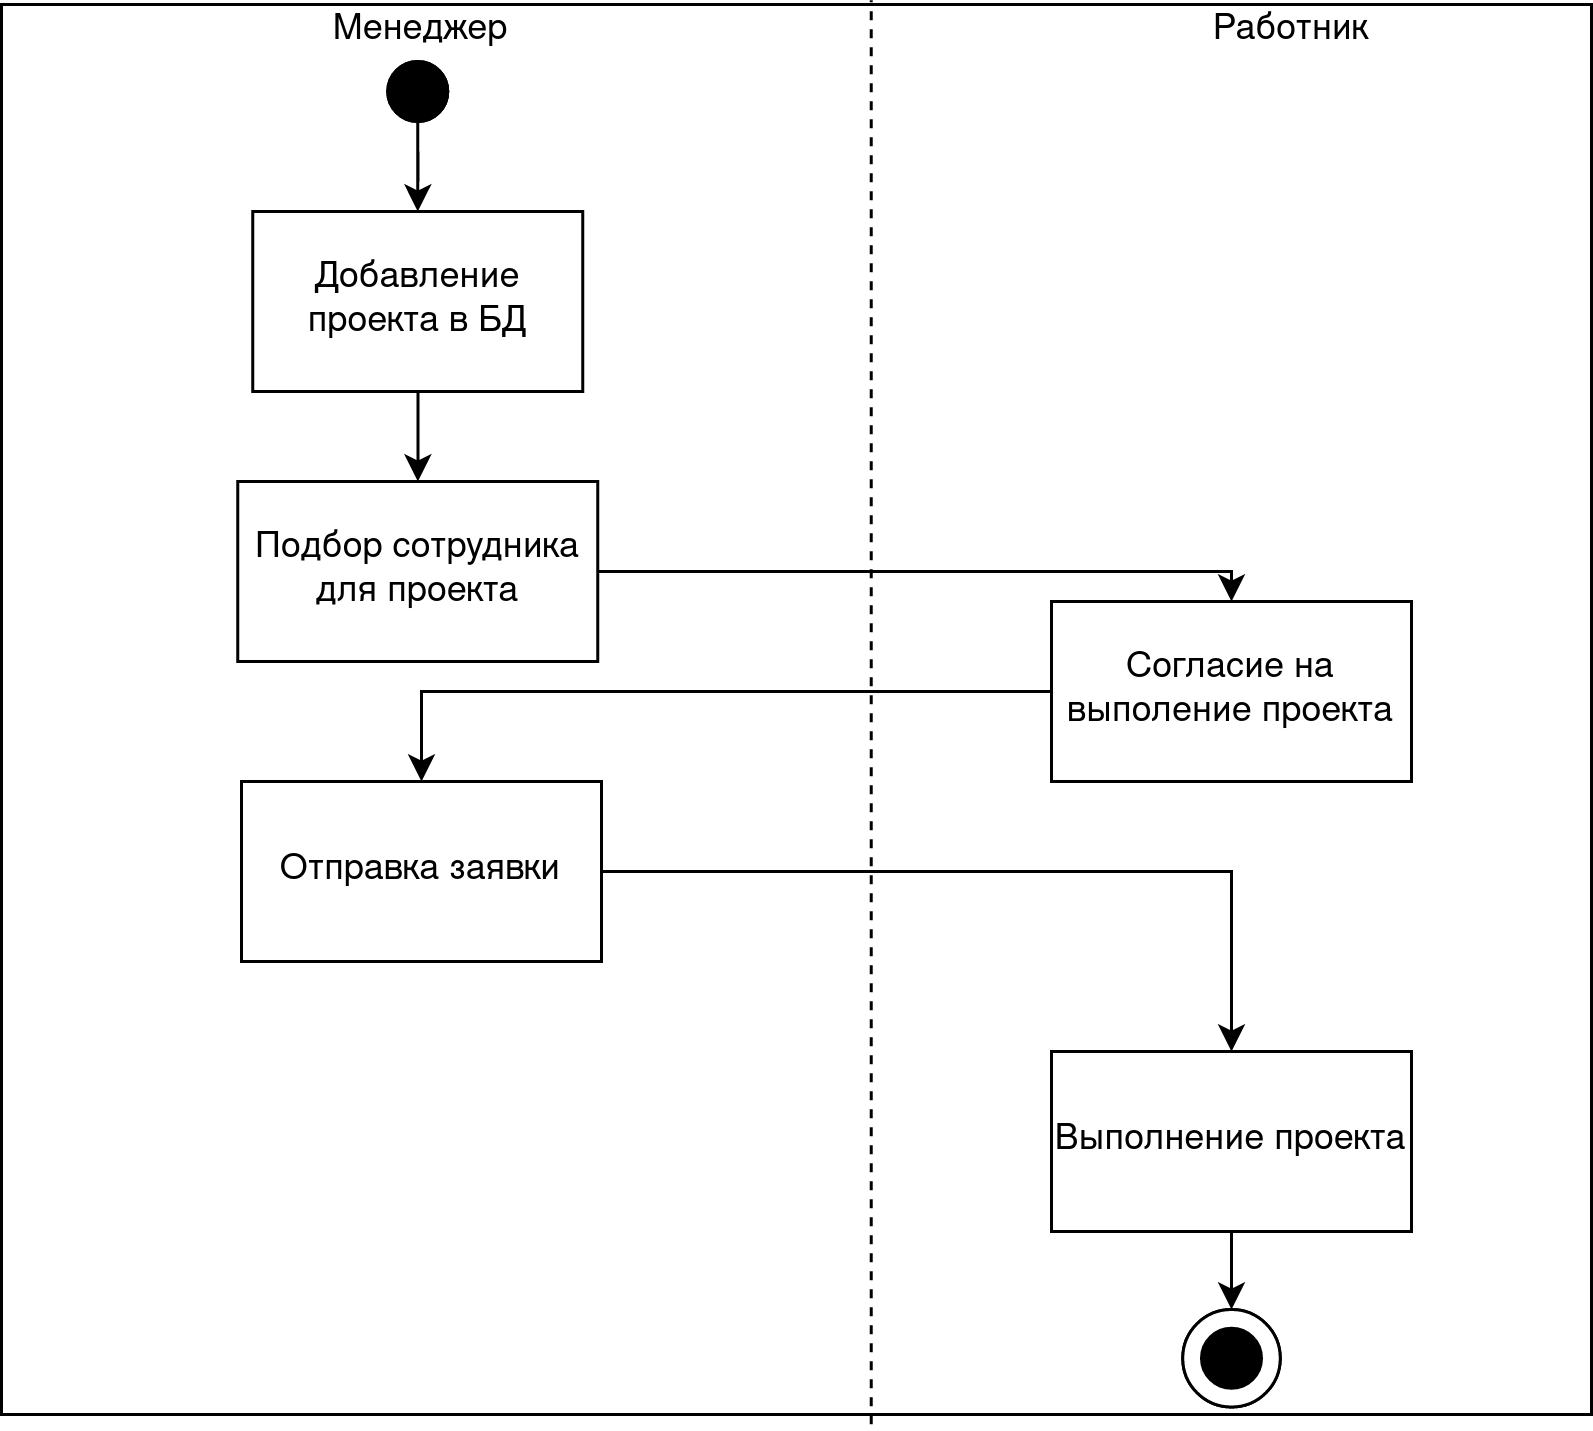
\includegraphics[width=0.4\textwidth]{img/Диаграмма Бизнес-процесса 1}
\end{FIGURE}
\subsection{Прецедента <<Редактирование информации об исполнителе>>}
Редактирование данных исполнителя.
\subsection{Описание прототипа}
Основной целью данной работы является проверка гипотезы об автоматическом поиске исполнителя на основании анализа текстов ВКР. Поэтому будет разрабатываться прототип, который будет включать в себя только следующие функции:
\begin{FIGURE}[h]{Диаграмма вариантов использования \label{fig:figure3}}
	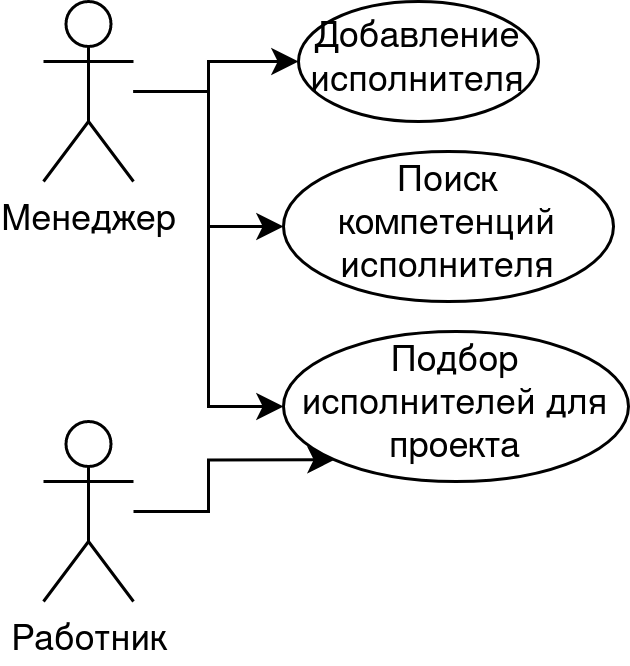
\includegraphics[width=0.4\textwidth]{img/Диаграмма вариантов использования прототипа}
\end{FIGURE}
\begin{itemize}
	\item Добавление исполнителей
	\item Поиск компетенций исполнителей
\end{itemize}
\section{Выбор языка программирования}
Для прототипирования подходят многие языки программирования, вот некоторые из них: Python, C\#, Java, JavaScript. Определимся с основными критериями для выбора языка:

\begin{itemize}
	\item Библиотеки для обучения моделей. Для работы с моделями машинного обучения.
	\item Предобученные модели. Так как для обучения модели надо иметь большой объем данных и много вычислительных мощностей.
	\item Библиотеки для обработки сайта.
	\item Библиотека для обработки docx и pdf файлов и обработки сайтов.
	\item Интерактивный режим. Позволяет просмотреть данные, преобразовать их, вмешаться в исполнение кода. Выполнить в произвольном порядке.
\end{itemize} 

\begin{TABLE}[!h]{Таблица сравнения языков программирования \label{tbl:tableProg}}
	\begin{tabular}[c]{|p{3cm}|p{2cm}|p{3cm}|p{2cm}|p{2cm}|p{3cm}|}
		\hline
		Язык программирования & Библиотека для МО & Предобученные модели & Работа с сайтом & Работа с файлами & Интерактивный режим\\ \hline
		Python 		& ++ & ++ & + & + & + \\ \hline
		C\# 		& +  & +  & + & + & - \\ \hline
		Java 		& +  & +  & + & + & - \\ \hline
		JavaScript 	& +  & +  & + & + & ? \\ \hline
	\end{tabular}
\end{TABLE}

Под эти критерии подходит Python. Он простой для написание и отладки, так как это интерпретируемый язык программирования, у него есть интерактивный режим. Также есть фреймворк PyThorch и библиотека с предобученными моделями HuggingFace Transformers, в частности RuBERT \cite{kuratov2019adaptation}, а также есть библиотека Bert Extractive Summarizer \cite{miller2019leveraging} для удобной работы с моделей.

\section{Выбор СУБД}
Для Python существуют библиотеки для работы с любыми системами управления базами данных. Для курсовой работы был выбран SQLite потому что его легко настраивать, нет необходимости устанавливать ничего дополнительно, что достаточно для прототипирования с небольшим количеством данных: 300 сотрудников и 1700 выпускных квалификационных работ.
\chapter{Проектирование системы}
\section{Проектирование базы данных}
Для разработки системы необходимо хранить информации о сотрудниках и выпускных квалификационных работах, где они были руководителями была разработана база данных. Необходимо было хранить:

\begin{description}
	\item [Код сотрудника] -- уникальный код сотрудника для его идентификации в базе данных
	\item [ФИО сотрудника] -- фамилия имя и отчество сотрудника
	\item [Ссылка на профиль сотрудника] -- ссылка на профиль сотрудника на сайте Высшей школы экономики, для последующей проверки в ручную при подборе на тендер
	\item [Код статуса] -- код статуса для последующей связи в базе данных
	\item [Код кафедры] -- код кафедры для последующей связи в базе данных
	\item [Компетенции] -- компетенции сотрудника полученные путём автоматического анализа текстов ВКР в текстовом виде
	\item [Эмбеддинги] -- компетенции сотрудника полученные путём автоматического анализа текстов ВКР в векторном пространстве для дальнейшего подбора исполнителя для тендера
	
	\item [Код статуса] -- уникальный код статуса для идентификации в базе данных
	\item [Наименования статуса] -- доцент, старший научный сотрудник и тд. Для представление информации о сотрудника.
	
	\item [Код кафедры] -- уникальный код кафедры для идентификации в базе данных
	\item [Наименование кафедры] -- название кафедры, где работает сотрудник. Для представление информации о сотруднике.
	
	\item [Код кампуса] -- уникальный код для идентификации в базе данных
	\item [Наименования кампуса] -- название кампуса. Для представление информации о сотруднике.
	
	\item [Код ВКР]  -- уникальный код выпускной квалификационной работы для идентификации в базе данных
	\item [Название ВКР] -- название выпускной квалификационной работы. Необходимо для дальнейшего соотнесения в сотрудника ручном режиме
	\item [Научный руководитель] -- код сотрудника для последующей связи в базе данных
	\item [Ссылка на ВКР] -- ссылка на выпускную квалификационную работу на сайте ВШЭ для проверки корректности сбора информации
	\item [Ссылка на полный текст ВКР] -- ссылка на файл для загрузки с полным текстом ВКР
	\item [ФИО студента] -- фамилия имя и отчество студента написавшего ВКР
	\item [Код ОП студента] -- код образовательной программы студента для последующей связи в базе данных
	\item [Код кампуса] -- код кампуса для последующей связи в базе данных
	
	\item [Код образовательной программы] -- уникальный код для идентификации в базе данных
	\item [Код факультета] -- код факультета для последующей связи в базе данных
	\item [Наименование ОП] -- название образовательной программы, где обучается студент
	
	\item [Код факультета] -- уникальный код факультета для идентификации в базе данных
	\item [Наименование факультета] -- название факультета
\end{description} 
Описание данных для проектирования БД \ref{tbl:tableDB}.
\begin{TABLE}[!h]{Таблица атрибутов \label{tbl:tableDB}}
	\begin{tabular}[c]{|p{4cm}|l|p{3cm}|l|p{3cm}|}
		\hline
		Имя атрибута & Тип данных & Значение по умолчанию & Формат ввода & Ограничение на значения\\ \hline

		Код сотрудника	 				& Число  & Нет & Нет 		& Нет \\ \hline
		ФИО сотрудника	 				& Строка & Нет & Нет 		& Нет \\ \hline	
		Ссылка на профиль сотрудника    & Строка & Нет & Нет 		& Нет \\ \hline
		Компетенции 					& Строка & Нет & Нет 		& Нет \\ \hline
		Эмбеддинги 						& Число  & Нет & Нет 		& Нет \\ \hline
		Код ВКР 						& Число  & Нет & Нет 		& Нет \\ \hline
		Название ВКР 					& Строка & Нет & Нет 		& Нет \\ \hline
		Ссылка на ВКР 					& Строка & Нет & Нет 		& Нет \\ \hline
		Ссылка на полный текст ВКР 		& Строка & Нет & Нет 		& Нет \\ \hline
		ФИО студента 					& Строка & Нет & Нет 		& Нет \\ \hline
		Код ОП студента 				& Число  & Нет & 00.00.00	& Нет \\ \hline
		Код статуса 					& Число  & Нет & Нет		& Нет \\ \hline
		Наименования статуса 			& Строка & Нет & Нет 		& Нет \\ \hline
		Код кафедры 					& Число  & Нет & Нет 		& Нет \\ \hline
		Наименование кафедры 			& Строка & Нет & Нет 		& Нет \\ \hline
		Код кампуса 					& Число  & Нет & Нет 		& Нет \\ \hline
		Наименования кампуса 			& Строка & Нет & Нет 		& Нет \\ \hline
		Код образовательной программы 	& Число  & Нет & 00.00.00 	& Нет \\ \hline
		Код факультета		 			& Число  & Нет & Нет 		& Нет \\ \hline
		Наименование ОП 				& Строка & Нет & Нет	 	& Нет \\ \hline
		Код факультета 					& Число  & Нет & Нет 		& Нет \\ \hline
		Наименование факультета 		& Строка & Нет & Нет 		& Нет \\ \hline
	\end{tabular}
\end{TABLE}
\subsection{Приведение к 1НФ}
Данные находятся в первой нормальной форме, если атрибуты атомарны и неделимы, состоят из элементарных составляющих и отсутствуют дубликаты.
\begin{enumerate}
	\item \underline{Код сотрудника}
	\item ФИО сотрудника
	\item Ссылка на профиль сотрудника
	\item Компетенции
	\item Эмбеддинги
	\item Код статуса сотрудника
	\item Код кафедры сотрудника
		
	\item \underline{Код ВКР}
	\item Название ВКР
	\item Код сотрудника
	\item Ссылка на ВКР
	\item Ссылка на полный текст ВКР
	\item ФИО студента
	\item Код кампуса
	\item Код ОП студента
	
	\item \underline{Код статуса}
	\item Наименование статуса
	
	\item \underline{Код кафедры}
	\item Наименование кафедры
	
	\item \underline{Код кампуса}
	\item Наименования кампуса
	
	\item \underline{Код образовательной программы}
	\item Код факультета
	\item Наименование ОП
	
	\item \underline{Код факультета}
	\item Наименование факультета
\end{enumerate} 

Данные атрибуты находятся в 1НФ.
\subsection{Приведение к 2НФ}
Данные находятся во второй нормальной форме, если они в первой нормальной форме и отсутствует частичная функциональная зависимость не ключевых атрибутов от ключа.
В соответствии с описанными выше зависимостями можно сделать вывод, что в описанном отношении имеются следующие частичные зависимости:
\begin{enumerate}
	\item Код сотрудника определяет:
	\begin{itemize}
		\item ФИО сотрудника
		\item Ссылка на профиль сотрудника
		\item Компетенции
		\item Эмбеддинги
		\item Код статуса сотрудника
		\item Код кафедры сотрудника
	\end{itemize}
	\item Код ВКР определяет:
	\begin{itemize}
		\item Название ВКР
		\item Код сотрудника
		\item Ссылка на ВКР
		\item Ссылка на полный текст ВКР
		\item ФИО студента
		\item Код кампуса
		\item Код ОП студента
	\end{itemize}
	\item Код статуса сотрудника определяет:
	\begin{itemize}
		\item Наименование статуса
	\end{itemize}
	\item Код факультета определяет:
	\begin{itemize}
		\item Наименование факультета
	\end{itemize}
	\item Код кампуса определяет:
	\begin{itemize}
		\item Наименование кампуса
	\end{itemize}
	\item Код кафедры определяет:
	\begin{itemize}
		\item Наименование кафедры
	\end{itemize}
	\item Код образовательной программы определяет:
	\begin{itemize}
		\item Название образовательной программы
	\end{itemize}
\end{enumerate}
\section{Сбор данных}
Для работы программы необходимо собрать данные о сотрудниках и ВКР, которые у них писались. Для этого надо было обрабатывать информация находящуюся на сайте ВШЭ. Такая обработка возможна с помощью библиотеки BeautifulSoap, который позволяет получать html любого сайта.

В первую очередь надо было получить список сотрудников и ссылки на их страницы. Для этого обрабатывался сайт со списком сотрудников, но там можно получить список сотрудников, фамилии которых начинаются на 1 букву. Что бы решить эту проблему с сайты получались ссылки на буквы. А потом с каждой такой ссылки собирался список сотрудников и ссылки на их страницы. Для этого брались все элементы страницы с атрибутом "a"\ и классом "link"\ , в которых значение атрибута "href"\ было "/org/persons/"\ или "/staff/". В базу данных записывались ФИО сотрудника и ссылку на их страницу. 

Далее надо было получить список ВКР для каждого сотрудника. Для этого брались все элементы страницы с атрибутом "a"\ и классом "link"\ , в которых значение атрибута "href"\ было "/edu/vkr/". Итого получилось собрать информацию о 321 сотруднике и 1708 ВКР.

Потом надо было получить информацию о ВКР, но их данные ВКР, в отличие от данных сотрудников, подгружались после загрузки основой страницы. Чтобы решить эту проблему пришлось эмулировать работу браузера с помощью библиотеки Selenium и драйвера Gecko (движок браузера FireFox). Библиотека Selenium не использовалась раньше, так как для ее работы надо больше времени и ресурсов, поэтому данная библиотека использовалась только на данном этапе. Для полной загрузки страницы ставилась задержка в 2 секунды. И бралась информация атрибута "p"\ с классом "vkr-card\_\_item". Также бралась информация о научном руководителе, он искался в базе данных, и потом в базу данных уже записывался Код сотрудника.

Чтобы получить тексты из файлов, они обрабатывались с помощью textract, которая позволяет получить информацию из pdf, doc и docx файлов, и помещались в базу данных.
\section{Создание компетентностного профиля исполнителя}
Для создание профиля человека рассматривались TFiDF \cite{das2018improved} и суммаризация текста c помощью BERT \cite{devlin2019bert} (Bidirectional Encoder Representations from Transformers). 

Подход TFiDF заключается в том что бы для каждого слова посчитать его отношение числа вхождений некоторого слова к общему числу слов документа (TF) и частоты, с которой некоторое слово встречается в документах коллекции (DF). Частоты в рамках коллекции рассматриваются для того что бы выявить распространённые слова в данных документах и снизить их важность, например "Информационная система", и наоборот найти слова которые находят важную тему, например "Машинное обучение".  Данный подход часто используется для кластеризации текстов. Но данный метод плохо подходит для данной задачи, потому что он не рассматривает контекст используемых слов. Это значит у него проблемы с омонимами и синонимами. Например, в предложениях "Ключ открыл замок" и "Рыцарь штурмовал замок" слова "зАмок" и "замОк" будут считаться как одно и тоже слово, хотя по контексту это разные слова.

BERT -- это нейросетевая языковая модель, которая рассматривает контекст, в котором находится слово и кодирует данное слово в своём векторном пространстве. Для этого модели подаётся на вход предложение, и каждое слово разделяется на отдельную часть предложения (токенизируется). Потом в начало и конец предложения добавляются специальные токены ([CLS], [SEP]), затем все токены предложения приводятся к нормальной форме слова (лемматизируются). Потом каждому слову присваивается вектор (эмбеддинг), которым кодируется слово. Для предложений также строится свой эмбединг. Цель работы данного алгоритма -- предсказывать следующее слово или понять идут предложения рядом или нет. Пример работы алгоритма \ref{fig:BERT sentences}. 

\begin{FIGURE}[h]{Обработка предложения \label{fig:BERT sentences}}
	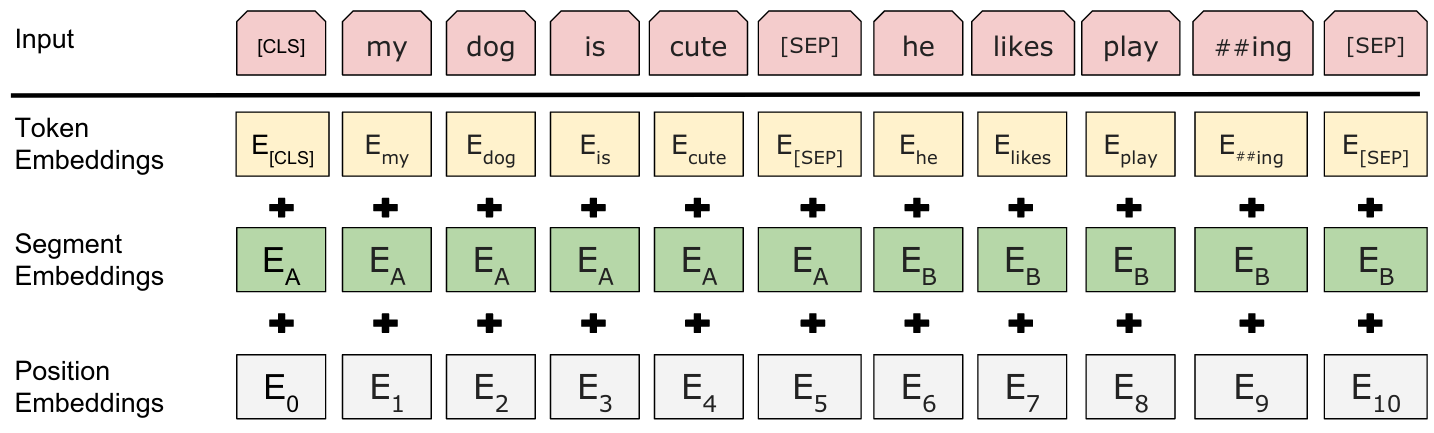
\includegraphics[width=0.6\textwidth]{img/BERT sentences}
\end{FIGURE}

При обучении задачи на предсказание следующего слова нейронная сеть закрывает 15\% слов маской, и пытается предсказывает какие слова были замаскированы на основе контекста. Для этого нейронная сеть находит вектора слов, которые находятся рядом в предложении, и берет близкое слово в векторном пространстве, относительно соседних слов \ref{fig:BERT illustrated}. 

\begin{FIGURE}[h]{Поиск "замаскированного" слова \label{fig:BERT illustrated}}
	\includegraphics[width=0.6\textwidth]{img/BERT illustrated}
\end{FIGURE}

В данной работе использовался предобученный BERT от DeepPavlovAI RuBert \cite{kuratov2019adaptation}, который обучался на русских текстах. 

Для задачи определения последовательности предложений в модель часть предложений поступает в последовательно, а другая часть в случайном порядке. И модель пытается предсказать какие из этих предложений находятся рядом в оригинальном тексте \ref{fig:BERT example}.

\begin{FIGURE}[h]{Схема работы BERT \label{fig:BERT example}}
	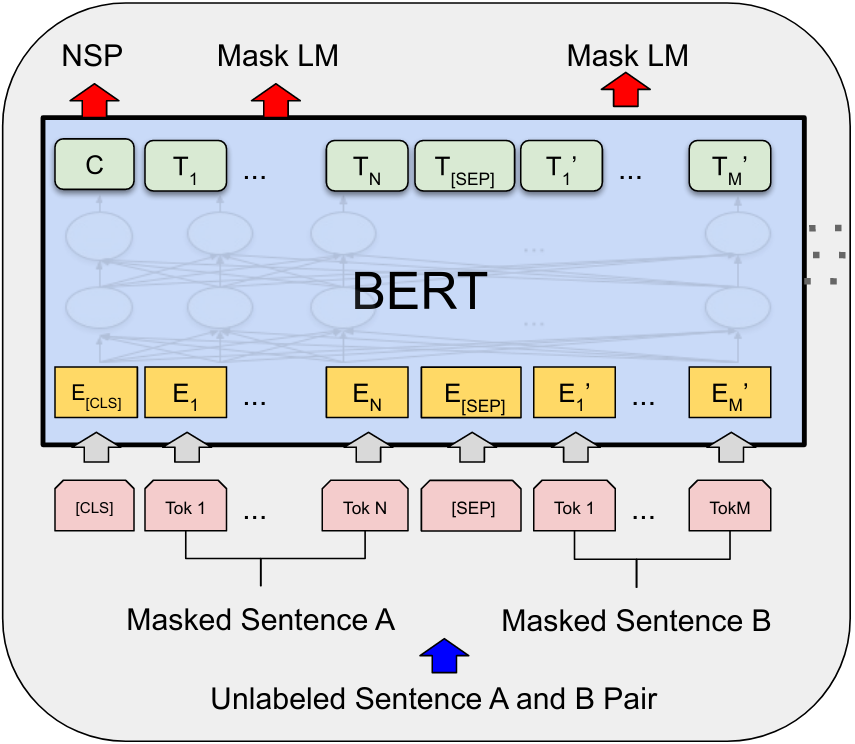
\includegraphics[width=0.6\textwidth]{img/BERT example}
\end{FIGURE}

BERT обрабатывал ВКР, которые написаны у сотрудников. С его помощью мы получили эмбединги предложений из ВКР. Получилось очень много предложений и надо получить короткое описание текстов фиксированного размера для каждого сотрудника. Чтобы сделать это можно взять самые типовые предложения, чем и занимается библиотека BERT Extractive summarizer \cite{miller2019leveraging}. 

BERT Extractive summarizer ищет эмбединги предложений, которые находятся рядом в векторном пространстве и объединяет их в группы (кластеры). И результатом общений текстов будет самое близкое предложение к центру кластера \ref{fig:Summ Knn}, что позволяет получить краткое содержание текста. Таким образом получается описание текста в виде эмбединга, для удобства работы алгоритмически, и текста, для проверки в ручную, остаётся сопоставить описание сотрудника и текстового задания.

\begin{FIGURE}[h]{Пример поиска содержания предложений \label{fig:Summ Knn}}
	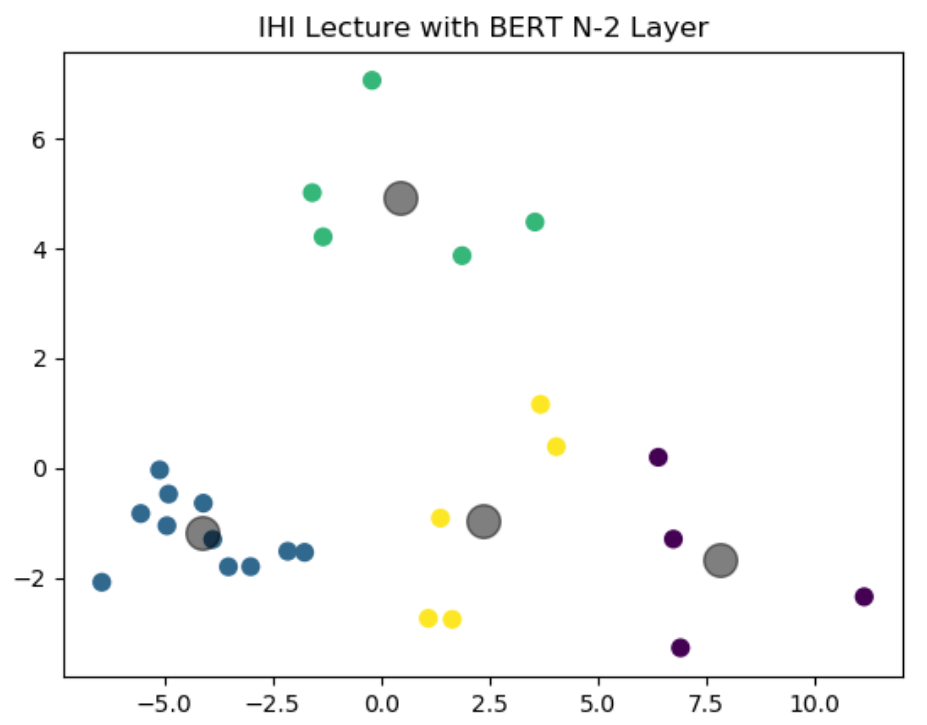
\includegraphics[width=0.6\textwidth]{img/Summ Knn}
\end{FIGURE}

\section{Возможные методы подбора исполнителя по ТЗ}
Для подбора исполнителя сравнивались эмбединнги текстового задания и сотрудника. Для лучшего подбора подходящего человека были разработаны разные функции поиска расстояний. Результатом работы алгоритма является исполнитель с наименьшим расстоянием между описанием задания и компетенциями исполнителя. Реализованные функции расчёта расстояний:
\begin{itemize}
	\item Средняя разница элементов -- в данном методе поиска расстояний, отрицательное расстояние может скомпенсировать положительное.
	\item Модуль разницы элементов (Манхэтонновское расстояние) -- этот метод поиска расстояний будет штрафовать за расстояния, которые находятся близко сильнее, чем расстояние Евклида.
	\item Квадрат разницы элементов  (Евклидово расстояние) --  этот метод поиска расстояний будет штрафовать за расстояния, которые находятся далеко сильнее, чем Манэтонновское расстояние.
\end{itemize}
Нужно было сопоставить 10 эмбедингов текстового описания задания и 10 эмбедингов сотрудника. Для этого было реализовано несколько алгоритмов:
\begin{itemize}
	\item Все со всеми. Каждый эмбединг текста сопоставляется с эмбеднигами сотрудника и считается сумма их расстояний.
	\item Поиск минимального с повторами. Для каждого эмбеддинга текста находится минимальное расстояние с эмбедингом сотрудника и считается сумма каждой такой пары.
	\item Поиск минимального без повторов. Для каждого эмбеддинга текста находится минимальное расстояние с эмбедингом сотрудника, если уже была пара с таким эмбедингом сотрудника, то берётся другой эмбединг с минимальный расстоянием, и считается сумма каждой такой пары.
	\item Усреднение эмбеддингов. Эмбеддинги сотрудника и текста усредняются и считается расстояние между ними.
\end{itemize}
Cхемы подбора находятся в Приложении А.
\chapter{Разработка и тестирование системы}
\section{Разработка интерфейсов}
Для удобства был сделан графический интерфейс \ref{fig:GUI}. С помощью него можно ввести текстовое описание задачи и подобрать походящего исполнителя.
\begin{FIGURE}[h]{Интерфейс приложения \label{fig:GUI}}
	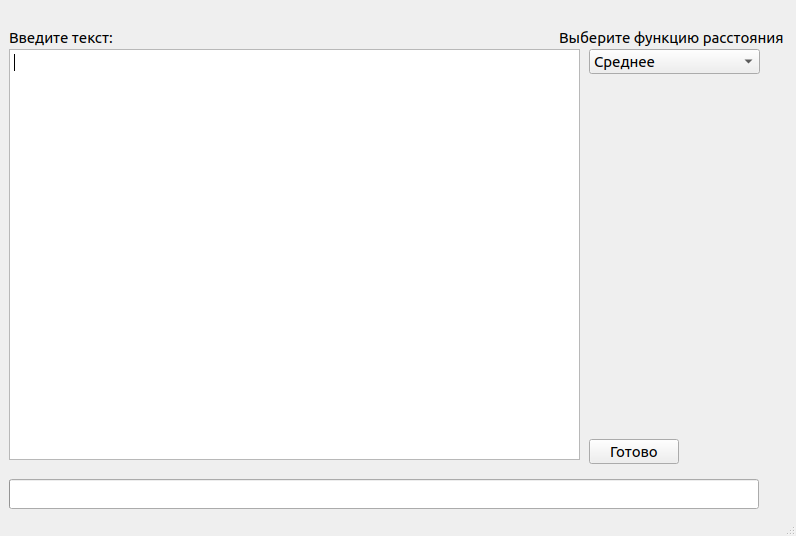
\includegraphics[width=0.6\textwidth]{img/GUI}
\end{FIGURE}

На данном окне есть текстовое поле куда вносится весь текст задания.

Для выбора функции ошибки есть ComboBox, в котором можно выбрать одну из следующих функций ошибки:
\begin{itemize}
	\item Среднее расстояние
	\item Манхэтонновское расстояние
	\item Евклидово расстояние
\end{itemize}

При нажатии кнопки Готово начинается подбор исполнителя, это занимает в среднем примерно 5 минут, для удобства отслеживания времени работы алгоритма был добавлен ProgressBar в низ приложения.

\section{Тестирование приложения}
Для тестирования приложения была выбрана выпускная квалификационная работа Абросимовой П. С. с темой <<Разработка средств автоматизации расширения онтологии на основе данных интернет-источников>> руководителем была Лядова Л. Н. Для тестирования в коде было сделано так чтобы, данный научный сотрудник не был решением алгоритма. Результаты работы разных алгоритмом и функций расстояния \ref{tbl:tableRes}.

\begin{TABLE}[!h]{Результатов работы программы \label{tbl:tableRes}}
	\begin{tabular}[c]{|p{4cm}|l|p{4cm}|l|}
		\hline
		Тип алгоритма        			& Среднее расстояние & Манхэттоновское расстояние & Расстояние Евклида \\ \hline
		Все со всеми		            & Кычкин А. В.       & Кушев В. О.                & Кушев В. О.        \\ \hline
		Поиск минимального с повторами  & Божья-Воля А. А.   & Кычкин А. В.               & Кычкин А. В.       \\ \hline
		Поиск минимального без повторов & Божья-Воля А. А.   & Божья-Воля А. А.           & Божья-Воля А. А.   \\ \hline
		Усреднение эмбеддингов      	& Кычкин А. В.       & Кузнецов Д. Б.             & Кузнецов Д. Б.     \\ \hline
	\end{tabular}
\end{TABLE}

Получилось 4 сотрудника Кычкин А. В., Кушев В. О., Божья-Воля А. А., Кузнецов Д. Б., из которых 3 сотрудника работают на кафедре информационных технологий в бизнесе и похожей сферой интересов с Лядова Л. Н.
\chapter*{Заключение}
В данной работе была разработана информационная система, целью которой было проверить гипотезу о том можно ли подобрать исполнителя под текстовое описание тендера.

Для этого было проведено проектирование и развёртывание базы данных. На основании базы данных была разработана и реализована информационная система, с помощью которой собирались данные с сайта ВШЭ и заполнились профили сотрудников НИУ ВШЭ.

Лучший результат показало расстояние Евклида.

В рамках работы в систему были загруженные реальные данные. Дальше было проведено тестирование и было показано, что разные функции тестирования дают разные результаты.

На основании текстового описания был произведён поиск путём расчёта расстояния между подаваемым текстом и профилем сотрудников. Было предложено несколько методов расчёта этого расстояния и было показано, что расстояние эвклида показало лучшее качество работы на нескольких примерах. На основании разработанной системы в дальнейшем требуется провести более детальное исселедование функций расстояния и выбрать ту, которая покажет наилучшее качество на большой выборке данных.
\putbibliography %Вместо этой команды будет вставлена библиография

\chapter*{ПРИЛОЖЕНИЕ A}
\begin{FIGURE}[h]{Все со всеми \label{fig:Подбор исполнителя 1}}
	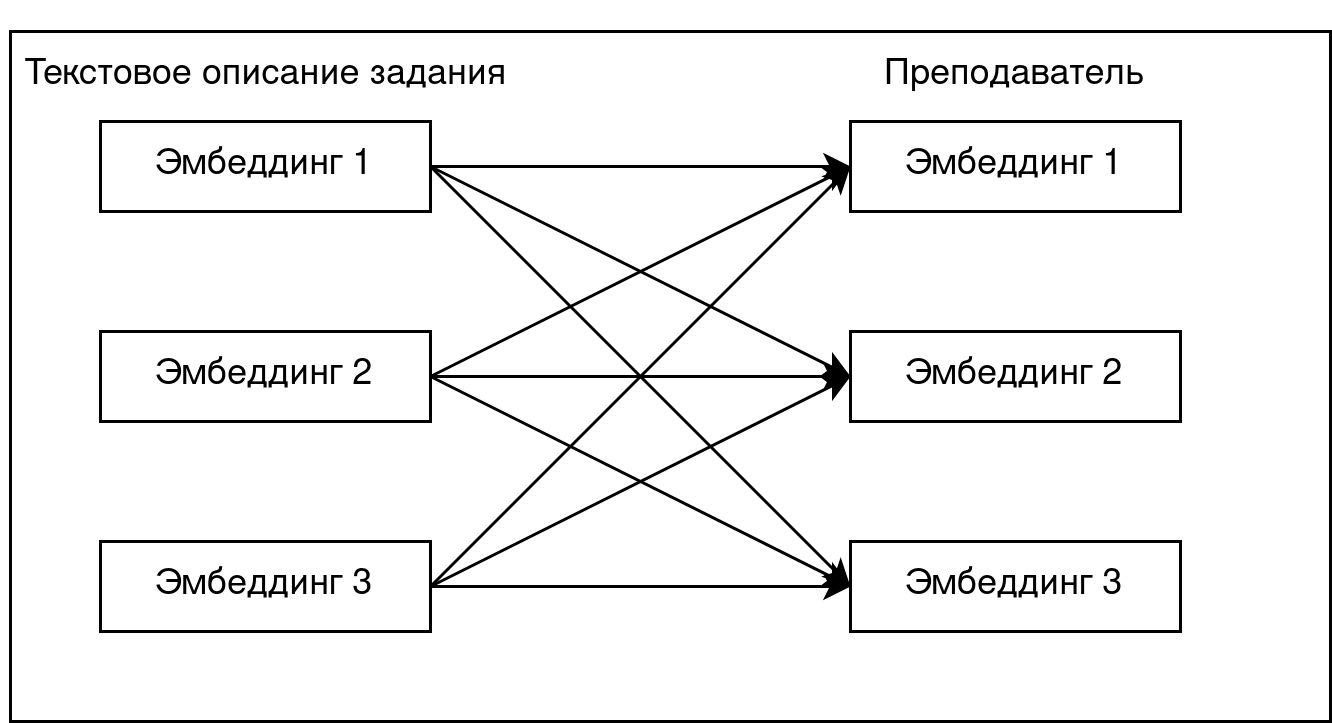
\includegraphics[width=0.6\textwidth]{img/Подбор исполнителя 1}
\end{FIGURE}
\begin{FIGURE}[h]{Поиск минимального с повторами \label{fig:Подбор исполнителя 2}}
	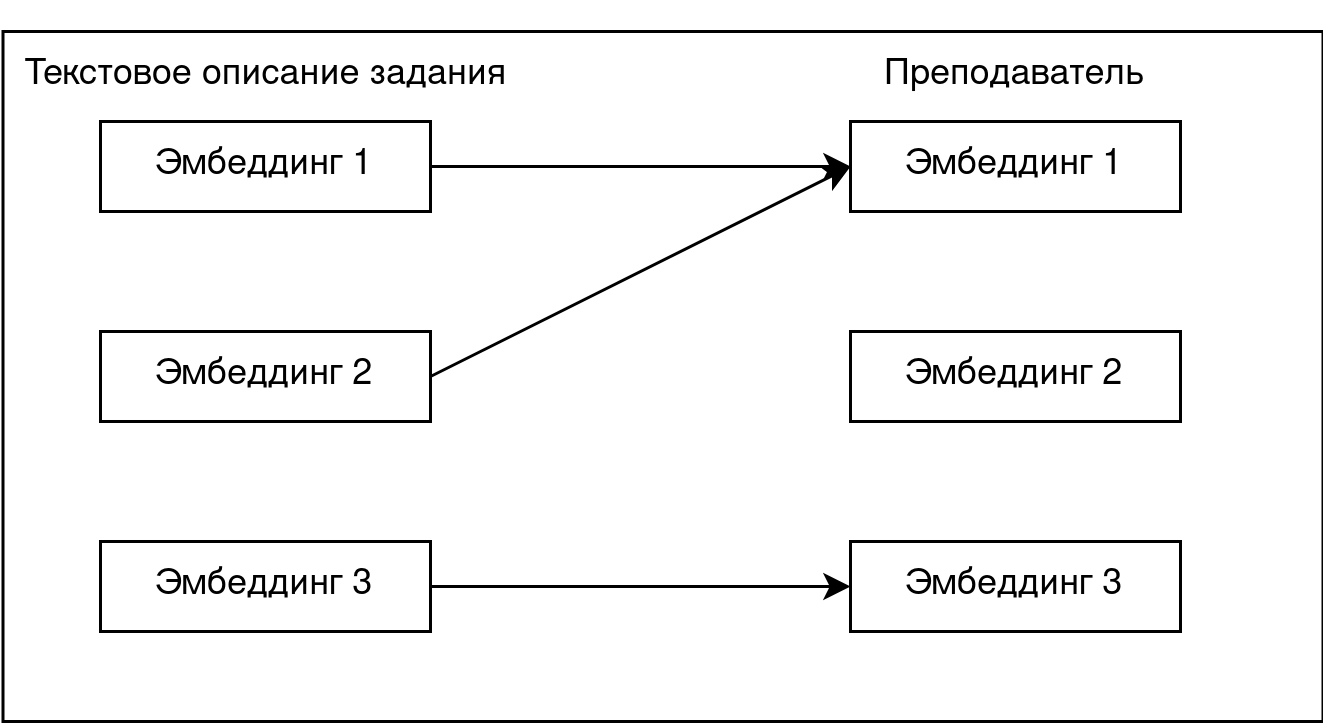
\includegraphics[width=0.6\textwidth]{img/Подбор исполнителя 2}
\end{FIGURE}
\begin{FIGURE}[h]{Поиск минимального без повторов \label{fig:Подбор исполнителя 3}}
	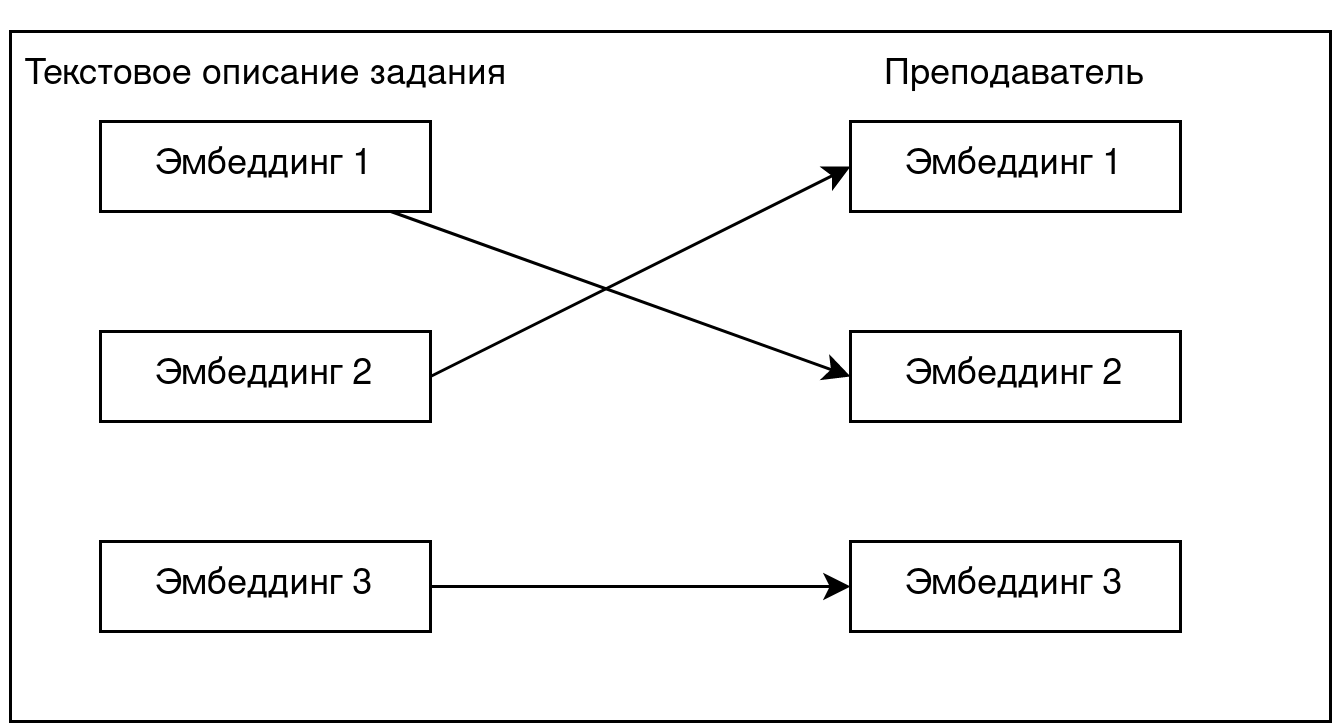
\includegraphics[width=0.6\textwidth]{img/Подбор исполнителя 3}
\end{FIGURE}
\begin{FIGURE}[h]{Усреднение эмбеддингов \label{fig:Подбор исполнителя 4}}
	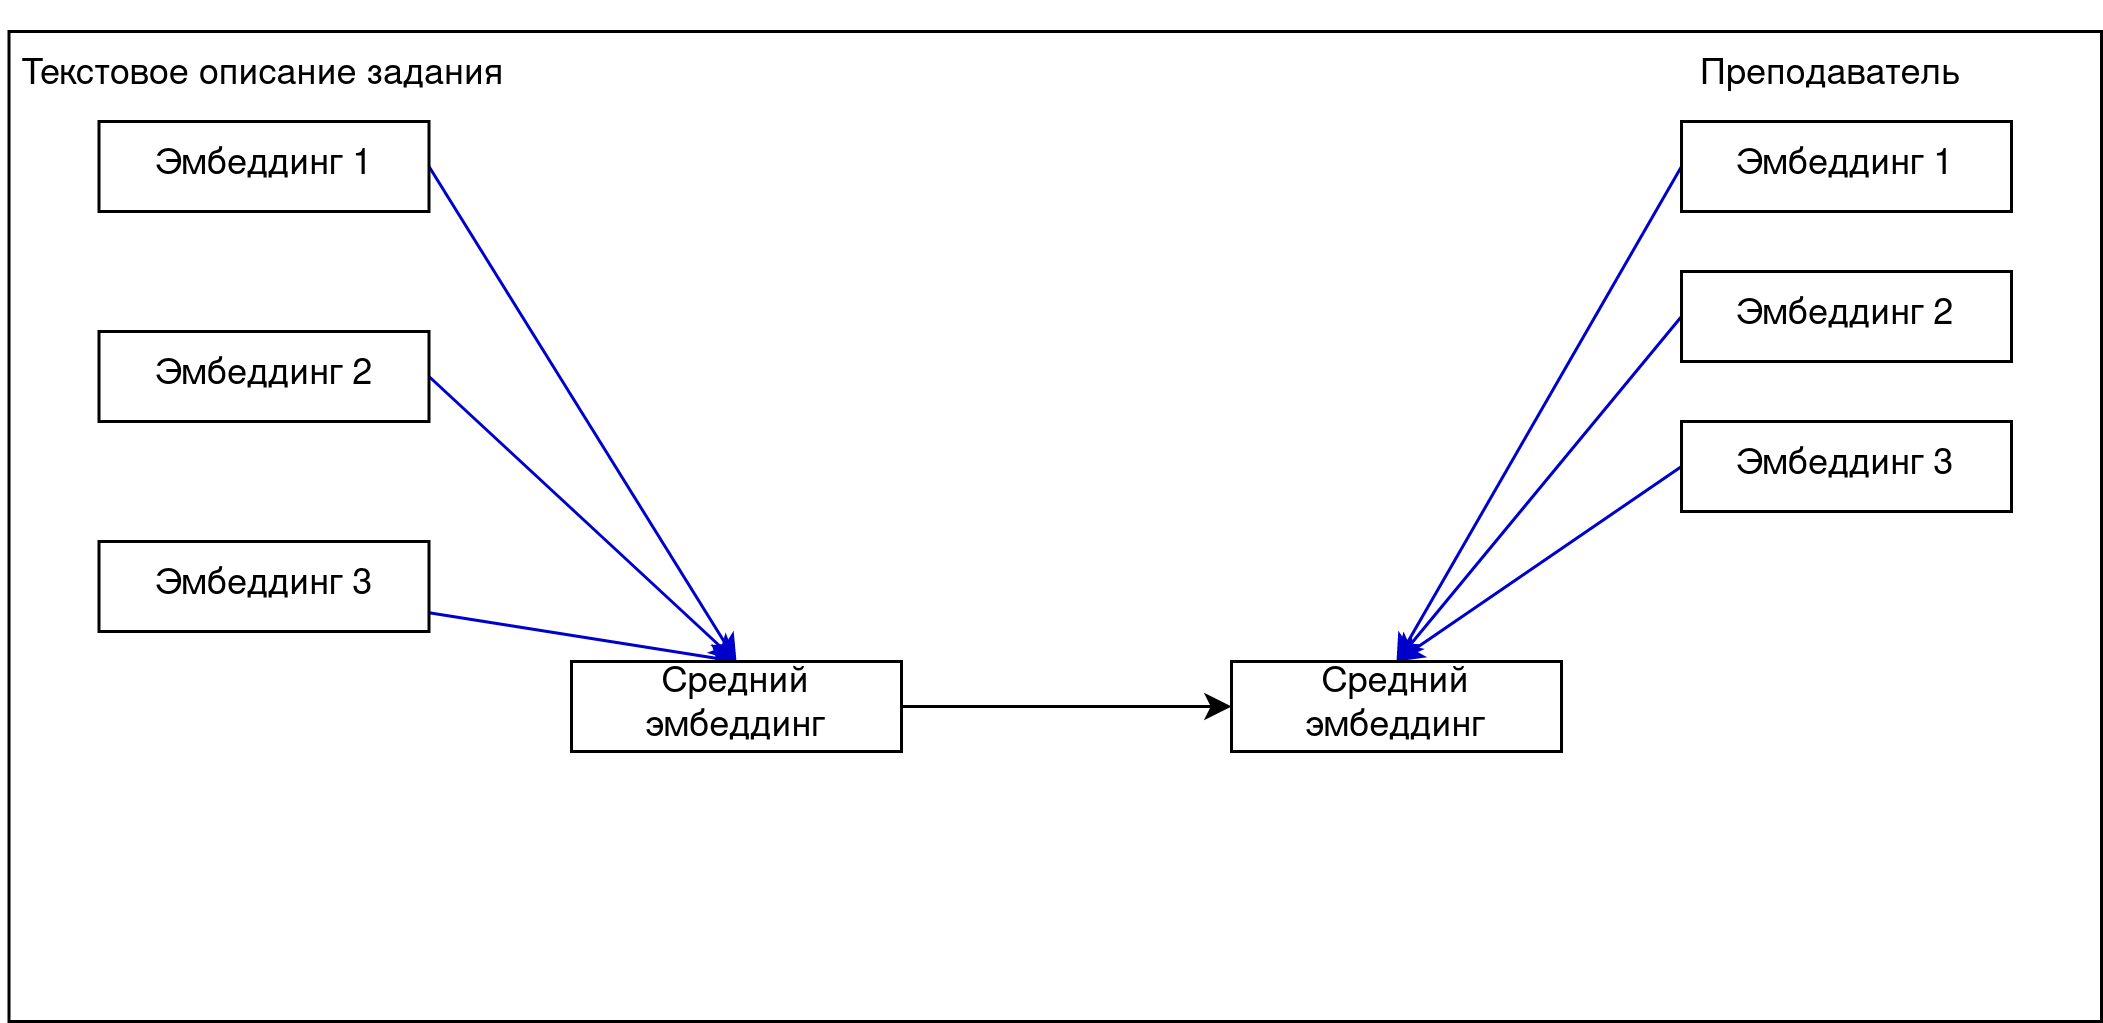
\includegraphics[width=0.6\textwidth]{img/Подбор исполнителя 4}
\end{FIGURE}
\end{document}
